\documentclass{sigchi}

% Use this command to override the default ACM copyright statement (e.g. for preprints). 
% Consult the conference website for the camera-ready copyright statement.


%% EXAMPLE BEGIN -- HOW TO OVERRIDE THE DEFAULT COPYRIGHT STRIP -- (July 22, 2013 - Paul Baumann)
% \toappear{Permission to make digital or hard copies of all or part of this work for personal or classroom use is 	granted without fee provided that copies are not made or distributed for profit or commercial advantage and that copies bear this notice and the full citation on the first page. Copyrights for components of this work owned by others than ACM must be honored. Abstracting with credit is permitted. To copy otherwise, or republish, to post on servers or to redistribute to lists, requires prior specific permission and/or a fee. Request permissions from permissions@acm.org. \\
% {\emph{CHI'14}}, April 26--May 1, 2014, Toronto, Canada. \\
% Copyright \copyright~2014 ACM ISBN/14/04...\$15.00. \\
% DOI string from ACM form confirmation}
%% EXAMPLE END -- HOW TO OVERRIDE THE DEFAULT COPYRIGHT STRIP -- (July 22, 2013 - Paul Baumann)


% Arabic page numbers for submission. 
% Remove this line to eliminate page numbers for the camera ready copy
\pagenumbering{arabic}


% Load basic packages
\usepackage{balance}  % to better equalize the last page
\usepackage{graphics} % for EPS, load graphicx instead
\usepackage{times}    % comment if you want LaTeX's default font
\usepackage{url}      % llt: nicely formatted URLs

% llt: Define a global style for URLs, rather that the default one
\makeatletter
\def\url@leostyle{%
  \@ifundefined{selectfont}{\def\UrlFont{\sf}}{\def\UrlFont{\small\bf\ttfamily}}}
\makeatother
\urlstyle{leo}


% To make various LaTeX processors do the right thing with page size.
\def\pprw{8.5in}
\def\pprh{11in}
\special{papersize=\pprw,\pprh}
\setlength{\paperwidth}{\pprw}
\setlength{\paperheight}{\pprh}
\setlength{\pdfpagewidth}{\pprw}
\setlength{\pdfpageheight}{\pprh}

% Make sure hyperref comes last of your loaded packages, 
% to give it a fighting chance of not being over-written, 
% since its job is to redefine many LaTeX commands.
\usepackage[pdftex]{hyperref}
\hypersetup{
pdftitle={SIGCHI Conference Proceedings Format},
pdfauthor={LaTeX},
pdfkeywords={SIGCHI, proceedings, archival format},
bookmarksnumbered,
pdfstartview={FitH},
colorlinks,
citecolor=black,
filecolor=black,
linkcolor=black,
urlcolor=black,
breaklinks=true,
}

% create a shortcut to typeset table headings
\newcommand\tabhead[1]{\small\textbf{#1}}


% End of preamble. Here it comes the document.
\begin{document}

\title{Glass Shooter: Exploring First-Person Shooter Game Design with Google Glass}

\numberofauthors{1} 
\author{\alignauthor Chun-Yen Hsu, Ying-Chao Tung, Silvia Chyou, Han-Yu Wang, Wei-Jer Lin, Mike Y. Chen \\
\affaddr{Mobile and HCI Research Lab, National Taiwan University} \\ 
\email{\{hcythomas0125,tony61507,silvia.chyou,huw12313212,evin92,belikemike\}@gmail.com}
}


\teaser{
\centering 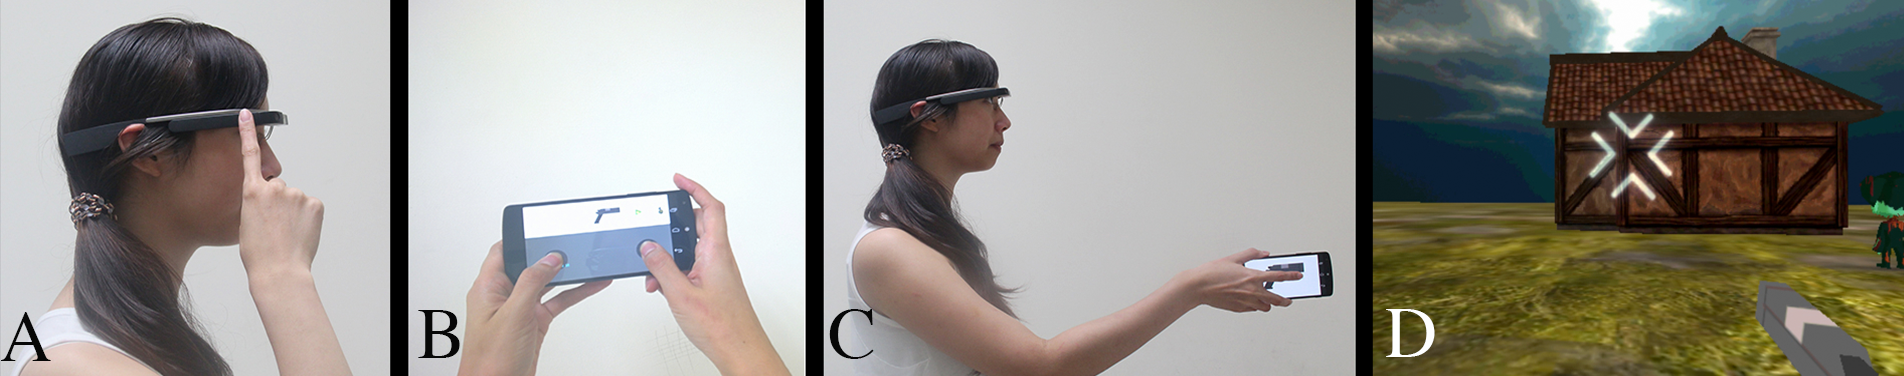
\includegraphics[width=1.0\textwidth]{GlassGame.png} 
\caption{(A) Glass Control: We designed a set of gestures on the strip touchpad. Players can move forward by pressing the front side of touchpad. By contrast, players can move back by pressing the back side of touchpad. Fire the weapon by a single tapping. Viewport is controlled by head orientation and scrolling the touchpad can also change the viewport direction; (B) Play with Controller: We use mobile phones to simulate game pad controllers. There are two joysticks on the phone. Left one controls avatar's movement while the right one rotates the direction of viewport. Players can tap anywhere to trigger the current weapon; (C) Play with Metaphor: The player holds the phone as a hand gun, manipulates the phone orientation to aim the target and triggers the gun by sliding the touch screen with a finger; (D) Game screenshot from Glass Shooter on Google Glass.}
\label{fig:figure1}
}

\maketitle



\begin{abstract}
Eyewear computers are claimed to be the next evolution beyond smart phones. In addition, game design for smart glasses game is still an unexplored area. Hence, we wish to explore the game design space on smart glasses. For testing the current game play experience on Google Glass, we recruited 24 users to play four games on Google Glass with different contents and control styles. By collecting users' imagination, we found about one third of users want to play a First-Person Shooter(FPS) game on the Google Glass. Hence, we implemented a FPS game on Google Glass and supply multiple control styles; (a) Glass control; (b) Play with controller; (c) Play with metaphor; to evaluate and explore glass game design.
\end{abstract}

\keywords{
	Google Glass, Wearable Devices, Game Design, Head Mounted Display, Multi-Modal, Mobile Phone, Gestures, Physical Activity, Mixed Reality, Augmented Reality, Virtual Reality. }
}

\category{K.8.0.}{Personal Computing}{General Games}


\section{Introduction}
Wearable devices are described as the next generation of smart devices because of their portability and computing power. One of the most significant wearable computing break-throughs is Google's new ``eyewear computer'', expecting to be commercially available in 2014 referred to as Glass~\cite{glass}. Due to the similarity between wearable devices and smart phones, many applications can be transferred to wearable devices, such as games. Recent statistics show that around 70-80\% of all mobile downloads is composed of mobile games\cite{statistics,infographic}. Traditional game design has tons of guidelines~\cite{videogame,mobilegame,bodygame,gameflow,argame,wearable}. However, it's lack of official research for smart glasses game design.% computers are claimed to be the next evolution beyond smartphones. 
%Game is one of the most important application in computer science.

Thus, we intend to explore the game design on smart glasses. Although there are several smart glasses products on the market over these years, we choose the most famous one, Google Glass, as our main research platform. To realize the current gameplay experience on google glass, we recruited 24 users to play 4 existing Google Glass games~\cite{minigame}, which has different game contents and control styles between each other. 
After analyzing users’ feedback, there are three novel issues, ``Limited control'', ``Eye tiring'' and ``Social acceptable'', which never exist in traditional game design guidelines. In our current work, we only focus on ``limited control''. Compared to other gaming platforms, there is no effective powerful input such as mouse, keyboard, joystick or touch screen. There are some non-traditional gaming inputs such as camera, strip touchpad, microphone, gyroscope, and accelerometer. How to design glass game in such a limited control device and how to extend its input power are open questions for people to discuss and explore. First, we ask users to imagine game type which they liked the most. According to game imagination results of users, one second of users want to play First-Person Shooter(FPS) game on Google Glass. Therefore, we implement a FPS game,``Glass Shooter'', with multiple control styles to explore glass game design space and understand user preference.

%Eyewear computers, such as google glasses implementation, are claimed to be the next evolution beyond smartphones. In addition, game industry in the US earned about 21.53 dollars in 2014\cite{essentialfacts}. Recent statistics show that around 70-80\% of all mobile downloads is composed of mobile games\cite{statistics,infographic}. Traditional game design has tons of guidelines\cite{videogame,mobilegame,bodygame,gameflow,argame,wearable}. However, the game design for smart glass game is still an unexplored area. Hence, we want to explore the game design space on smart glass. And after concerning current market share, we choose Google Glass as our candidate.

%First we want to realize the current game play experience on google glass, so we recruited 24 users to play existing google glass game\cite{minigame} with different content or control style. After user study, we found that about one third of users want to play First-Person Shooter(FPS) game on google glass. So we decide to implement a FPS game on google glass for demonstration. In addition, we also provide multiple control styles to evaluate and find out the best control way on google glass. 

\section{Game Prototype}
%To get deeper understanding of glass game design, we implement a game by ourselves, which called ``Glass Shooter'', so that we can have some control variable to change directly by ourselves and compare with different settings.
We choose FPS as our game type because 50\% of users prefer to play this kind of games on Google Glass according to our previous user study. There are many control issues in FPS games because of their multidimensional input requirements. To get deeper research of glass design, we implemented our own game, ``Glass Shooter'', a FPS game with multiple control choices to compare different input methods on the Google Glass. We expect that our FPS game can satisfy most users and get useful knowledge by studying and implementing this type of game.

\section{Game Control Style}
In our game control design, we also include the smart phone as a controller to increase the diversity of input manners. With these two different types of devices, they can complement each other to make up their own deficiencies. We totally designed three different control styles; (a) Glass Control; (b) Play with Controller; (c) Play with Metaphor. Although we present three different control styles, they are not completely conflict with each other, player can just use them together or switch between each style. We described the control styles below.


\subsection{Glass Control}
First we just focus on Google Glass itself. In glass control, the main control is composed of the built-in IMU(inertial measurement unit) sensors and the strip touchpad on the right side of the Google Glass.Viewport is controlled by head orientation. In addition, players can move forward by pressing the front side of touchpad. By contrast, players also can move back by pressing the back side of touchpad.
To avoid the huge variation of the direction of viewport, we present an optional method to control the viewport, players can scroll the touchpad to change the view direction. Furthermore, players can tilt right and left tilt to move the avatar and trigger their weapons by tapping the touchpad.%Scrolling the touchpad can also change the viewport direction, to avoid big degree of head rotation. Players can use left tilt and right tilt to move left and right. And by tapping on touchpad, players can trigger their weapons, such as a gun or a hand grenade. (see Figure~\ref{fig:figure1}A.)

\subsection{Play with Controller}
We design to use a smart phone as a game controller. Reference to traditional gamepad controller, there are two joysticks on the phone, left one controls the avatar's movement, right one rotates the viewport direction. Players can tap anywhere on the touch screen to trigger the current weapon. %In this case, player can still use head orientation to control viewport.
(see Figure~\ref{fig:figure1}B.)

\subsection{Play with Metaphor}
To explore interaction between the Google Glass and the smart phone, we also tried several experimental controls with metaphor. For example, the user can hold the phone as a hand gun to manipulate the phone orientation to aim the target and fire the gun by sliding the touch screen with the index finger. Another metaphor is holding the phone as a hand grenade. The player can use throwing gesture to throw out the grenade. We also implement the metaphor of holding a knife, the player can brandish the phone to perform a knife attack.(see Figure~\ref{fig:figure1}C.)

%\subsubsection{Phone aiming}
% Aiming by using smart phone as a gun
%By using both of our hands, we can hold the smart phone with the same posture as we hold a gun. With this pose, we can switch our angle of view by revolving our body. And by using gyro, we can aim the target or the enemy by trimming our smart phone to shoot precisely. In other words, we can use smart phone as a aiming device, such as players using an electric torch or a gun.

%\subsubsection{Thrower}
% Using smart phone as body motion sensing
%Take Nintendo Wii for example, players movement can be detected precisely by the sensor. Although google glass can't have as strong sensor as Nintendo Wii, we still can detect some players' movement by our controller, smar phone. For instance, players hold the smart phone and can do throwing motion to simulate as throwing the hand grenade, and can make waving motion as waving the knife, and so on.

%\subsubsection{Driving simulation}
%While player driving the car, player use controller to emulate their motion as driving the car. It can indead raise players' game play experience greatly. So we can hold our controller, smart phone, as a steering wheel by both user's hand, and revolving the smart phone to emulate turning of the steering wheel.

%\subsubsection{Traditional joystick}
%To compare various of control method, we also provide traditional joystick for players on our controller, smart phone. By using traditional joystick, players can turning their angle of view and move their position directily.

\section{Conclusion}
In this demonstration, we presented a first-person shooter game based on our user feedback from existing glass games. To explore the glass gaming control, which is still an open question nowadays, we designed and implemented multiple control styles; (a) Glass Control; (b) Play with Controller; (c) Play with Metaphor; this work still lacks of system validation, so we are planning to perform a formal user study currently. Moreover, we are interested in ``Eye tiring'' and ``Social acceptable'' problems on Google Glass because these puzzles do not appear in earlier works about other mobile devices.
To explore the complete game design space on Google Glass, we will accomplish a series of user studies to evaluate these two issues we found in our previous study in the following months. 
%we hope our effort can inspire more glass game developers to develope more intuitive and suitable controls. With better gaming controls, we belive it can enhance glass game play experience significantly than before, and we also hope to be able to inspire more exploration of smart glasses gaming and spread game entertainment for more people.


\section{Acknowledgements}
We thank our advisor Prof. Mike Y. Chen and the faculty and staff of National Taiwan University. We should also like to express our gratitude towards all players and testers who have helped us in our many (buggy) iterations.

\balance

\bibliographystyle{acm-sigchi}
\bibliography{sample}
\end{document}
